\documentclass{article}
% Change "article" to "report" to get rid of page number on title page
\usepackage{amsmath,amsfonts,amsthm,amssymb}
\usepackage{setspace}
\usepackage{Tabbing}
\usepackage{fancyhdr}
\usepackage{lastpage}
\usepackage{extramarks}
\usepackage{chngpage}
\usepackage{soul,color}
\usepackage{graphicx,float,wrapfig}
\usepackage{multirow}

% In case you need to adjust margins:
\topmargin=-0.45in      %
\evensidemargin=0in     %
\oddsidemargin=0in      %
\textwidth=6.5in        %
\textheight=9.0in       %
\headsep=0.25in         %

% Homework Specific Information
\newcommand{\hmwkTitle}{Weekly Report I}
\newcommand{\hmwkClass}{}
\newcommand{\hmwkAuthorName}{Donglai\ Wei}


% Setup the header and footer
\pagestyle{fancy}                                                       %
\lhead{\hmwkAuthorName}                                                 %
\rhead{\firstxmark}                                                     %
\lfoot{\lastxmark}                                                      %
\cfoot{}                                                                %
\rfoot{Page\ \thepage\ of\ \pageref{LastPage}}                          %
\renewcommand\headrulewidth{0.4pt}                                      %
\renewcommand\footrulewidth{0.4pt}                                      %

% This is used to trace down (pin point) problems
% in latexing a document:
%\tracingall

%%%%%%%%%%%%%%%%%%%%%%%%%%%%%%%%%%%%%%%%%%%%%%%%%%%%%%%%\begin{enumerate}

% Some tools
\newcommand{\enterProblemHeader}[1]{\nobreak\extramarks{#1}{#1 continued on next page\ldots}\nobreak%
                                    \nobreak\extramarks{#1 (continued)}{#1 continued on next page\ldots}\nobreak}%
\newcommand{\exitProblemHeader}[1]{\nobreak\extramarks{#1 (continued)}{#1 continued on next page\ldots}\nobreak%
                                   \nobreak\extramarks{#1}{}\nobreak}%

\newlength{\labelLength}
\newcommand{\labelAnswer}[2]
  {\settowidth{\labelLength}{#1}%
   \addtolength{\labelLength}{0.25in}%
   \changetext{}{-\labelLength}{}{}{}%
   \noindent\fbox{\begin{minipage}[c]{\columnwidth}#2\end{minipage}}%
   \marginpar{\fbox{#1}}%

   % We put the blank space above in order to make sure this
   % \marginpar gets correctly placed.
   \changetext{}{+\labelLength}{}{}{}}%

\setcounter{secnumdepth}{0}
\newcommand{\homeworkProblemName}{}%
\newcounter{homeworkProblemCounter}%
\newenvironment{homeworkProblem}[1][Problem \arabic{homeworkProblemCounter}]%
  {\stepcounter{homeworkProblemCounter}%
   \renewcommand{\homeworkProblemName}{#1}%
   \section{\homeworkProblemName}%
   \enterProblemHeader{\homeworkProblemName}}%
  {\exitProblemHeader{\homeworkProblemName}}%

\newcommand{\problemAnswer}[1]
  {\noindent\fbox{\begin{minipage}[c]{\columnwidth}#1\end{minipage}}}%

\newcommand{\problemLAnswer}[1]
  {\labelAnswer{\homeworkProblemName}{#1}}

\newcommand{\homeworkSectionName}{}%
\newlength{\homeworkSectionLabelLength}{}%
\newenvironment{homeworkSection}[1]%
  {% We put this space here to make sure we're not connected to the above.
   % Otherwise the changetext can do funny things to the other margin

   \renewcommand{\homeworkSectionName}{#1}%
   \settowidth{\homeworkSectionLabelLength}{\homeworkSectionName}%
   \addtolength{\homeworkSectionLabelLength}{0.25in}%
   \changetext{}{-\homeworkSectionLabelLength}{}{}{}%
   \subsection{\homeworkSectionName}%
   \enterProblemHeader{\homeworkProblemName\ [\homeworkSectionName]}}%
  {\enterProblemHeader{\homeworkProblemName}%

   % We put the blank space above in order to make sure this margin
   % change doesn't happen too soon (otherwise \sectionAnswer's can
   % get ugly about their \marginpar placement.
   \changetext{}{+\homeworkSectionLabelLength}{}{}{}}%

\newcommand{\sectionAnswer}[1]
  {% We put this space here to make sure we're disconnected from the previous
   % passage

   \noindent\fbox{\begin{minipage}[c]{\columnwidth}#1\end{minipage}}%
   \enterProblemHeader{\homeworkProblemName}\exitProblemHeader{\homeworkProblemName}%
   \marginpar{\fbox{\homeworkSectionName}}%

   % We put the blank space above in order to make sure this
   % \marginpar gets correctly placed.
   }%

%%%%%%%%%%%%%%%%%%%%%%%%%%%%%%%%%%%%%%%%%%%%%%%%%%%%%%%%%%%%%



%%%%%%%%%%%%%%%%%%%%%%%%%%%%%%%%%%%%%%%%%%%%%%%%%%%%%%%%%%%%%
% Make title
\title{\vspace{0.3in}\textmd{\textbf{\hmwkTitle}}}
\date{2010.4.5}
\author{\textbf{\hmwkAuthorName}}
%%%%%%%%%%%%%%%%%%%%%%%%%%%%%%%%%%%%%%%%%%%%%%%%%%%%%%%%%%%%%

\begin{document}
\begin{spacing}{1.1}
\maketitle



  
\section{1. Comparison Among EE,collapsed EE and ME for DPmixture}
\subsection{1.1 Settings}


\begin{center}
 Graphical Model for DP mixture\\
    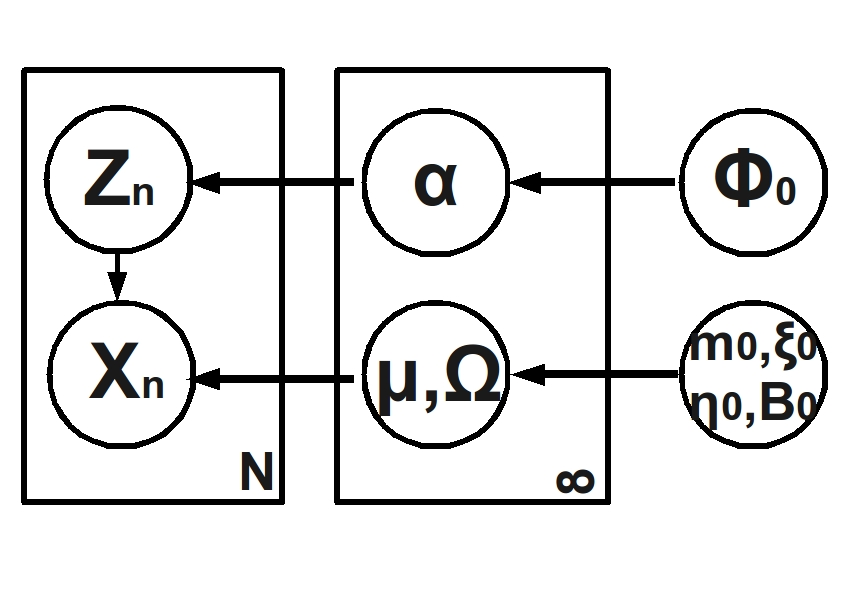
\includegraphics[width=3in,height=2in]{dp.jpg} 
\end{center}
 


\large {\bf 0) Notation:}\\
  $x_{n}$:observation;\\
  $z_{n}$:assignment;\\
  $\theta$:parameter \  (Hidden Variables besides $z_{n}:\alpha,\mu,\Omega$);\\
  hyper: hyper-parameters (Prior:$\phi_{0},m_{0},B_{0},\eta_{0},\xi_{0}$)\\ \\
\large {\bf 1) Conditional Probability:} \\
EE(stick-breaking):\\$p(x_{n},z_{n},\theta|hyper)=\mathcal{M}(z_{n}|\alpha^{'})\mathcal{B}(1,\phi_{0})\mathcal{N}(x_{n}|z_{n},\mu,\Omega)
\mathcal{N}(\mu|m_{0},\xi_{0}\Omega)\mathcal{W}(\Omega|\eta_{0},B_{0})$\\ \\
ME(limit of finite mixture):\\$p(x_{n},z_{n},\theta|hyper)=\mathcal{M}(z_{n}|\alpha)\mathcal{D}(\alpha|\phi_{0})\mathcal{N}(x_{n}|z_{n},\mu,\Omega)
\mathcal{N}(\mu|m_{0},\xi_{0}\Omega)\mathcal{W}(\Omega|\eta_{0},B_{0})$\\ \\
\large {\bf 2) Free Energy:} \\
$\mathcal{F}([z],K_{+})=\sum_{c=1}^{K_{+}}[\frac{DN_{c}}{2}log\pi+\frac{D}{2}log\frac{\xi_{c}}{\xi_{0}}log det(B_{c})
-\frac{\eta_{0}}{2}log det(B_{0})-log \frac{\Gamma_{D}(\frac{\eta_{c}}{2})}{\Gamma_{D}(\frac{\eta_{0}}{2})}$\\
\ \  \underline{ $+\frac{1}{K_{+}}log \frac{\Gamma(N+\phi_{0})}{\Gamma(\phi_{0})} -log(\Gamma(N_{c})-log \phi_{0}]$}

\subsection{1.2 Prior 1 (default ME(top-down))}
$\phi_{0}$=2\\
$m_{0}=\bar{x}$=(0.0217,1.6134)\\
$B_{0}$=b0r*D*S=[0.1505,0.0113;0.0113,0.2518] \\
$\eta_{0}$=2\\
$\xi_{0}$=0.1\\
(b0r=0.1151(random),D=2,S=[0.6536,0.0493;0.0493,1.0936](cov matrix))\\
(Algorithms are implemented by Kurihara,free energy threshold for EE,c-EE is 1e-10)
\begin{table}[t]
\caption{Prior 1 (with mean and std)}
\begin{center}
\begin{tabular}{|l|l|l|l|}

\hline
{\bf Learning Algorithm} &{\bf Initial Cluster Numbers} &{\bf Number of clusters}  &{\bf RandIndex} \\ 
\hline 
\multirow{2}{*}{EE(sampled initialization)} & 10 & 4.1(0.3) & 0.99(0.00) \\
					    & 20 & 4.1(0.3) & 0.99(0.00)\\
\hline
\multirow{2}{*}{EE(random initialization)}  & 10 & 4.4(0.48)&  0.97(0.01) \\
					    & 20 & 4.5(0.83)&  0.96(0.01) \\
\hline
\multirow{2}{*}{Collapsed EE}               & 10 & 5.0(1.0)&  0.97(0.22) \\
					    & 20 & 7.1(1.7)&  0.85(0.07) \\
\hline
\multirow{6}{*}{ME}                         & 1(Top-down) &    4  &  1 \\
					    & 200(Bottom-up) & 4  &  1 \\
					    & 200(Local search,1-200 update) & 6 &  0.91  \\
					    & 200(..+Merge) & 4   &  1 \\
					    & 200(Local search,random update) & 5.9(1.37)&  0.94(0.05) \\
					    & 200(..+Merge) & 4(0)&  1(0) \\
\hline
\end{tabular}
\end{center}
\end{table}


 \begin{center}
Prior 1: ME,1-200 update\\    
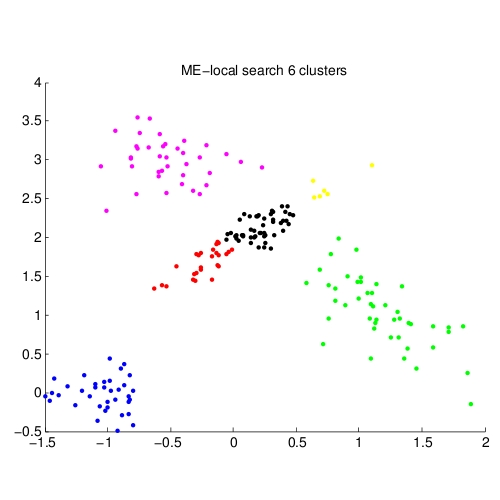
\includegraphics[width=4in,height=3.7in]{0_me_1.jpg}\\
Prior 1: ME,random update\\
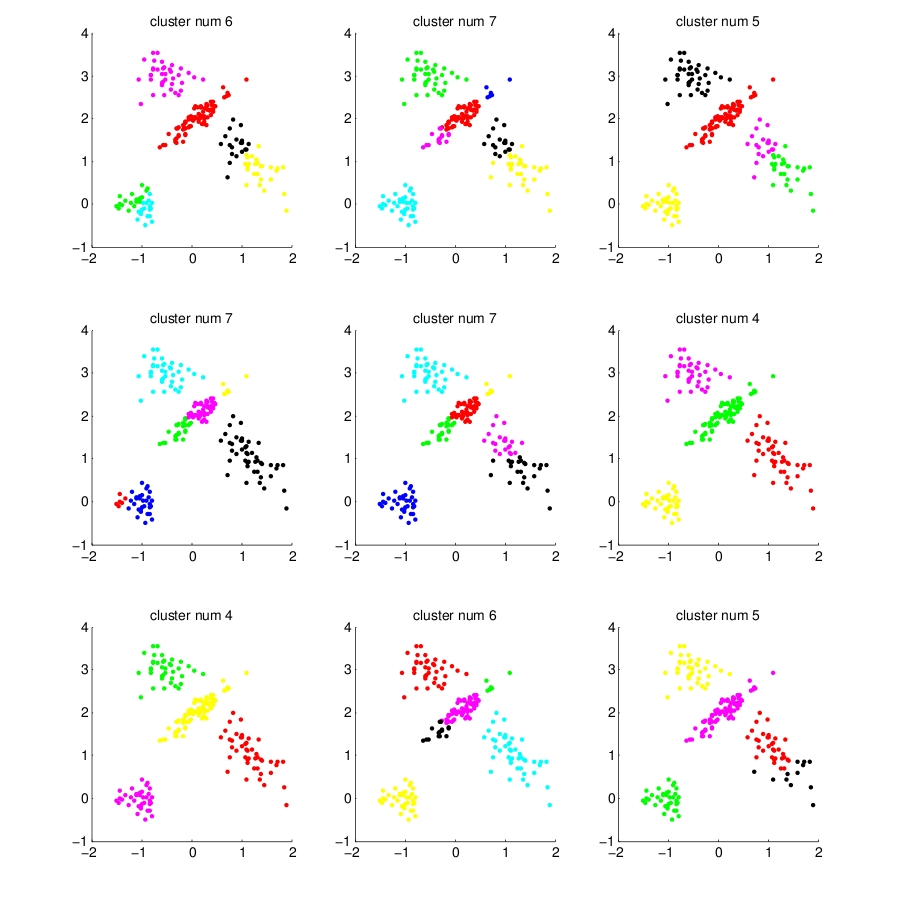
\includegraphics[width=5in,height=4.25in]{0_me_r.jpg} \\
Prior 1: c-EE,K=20\\
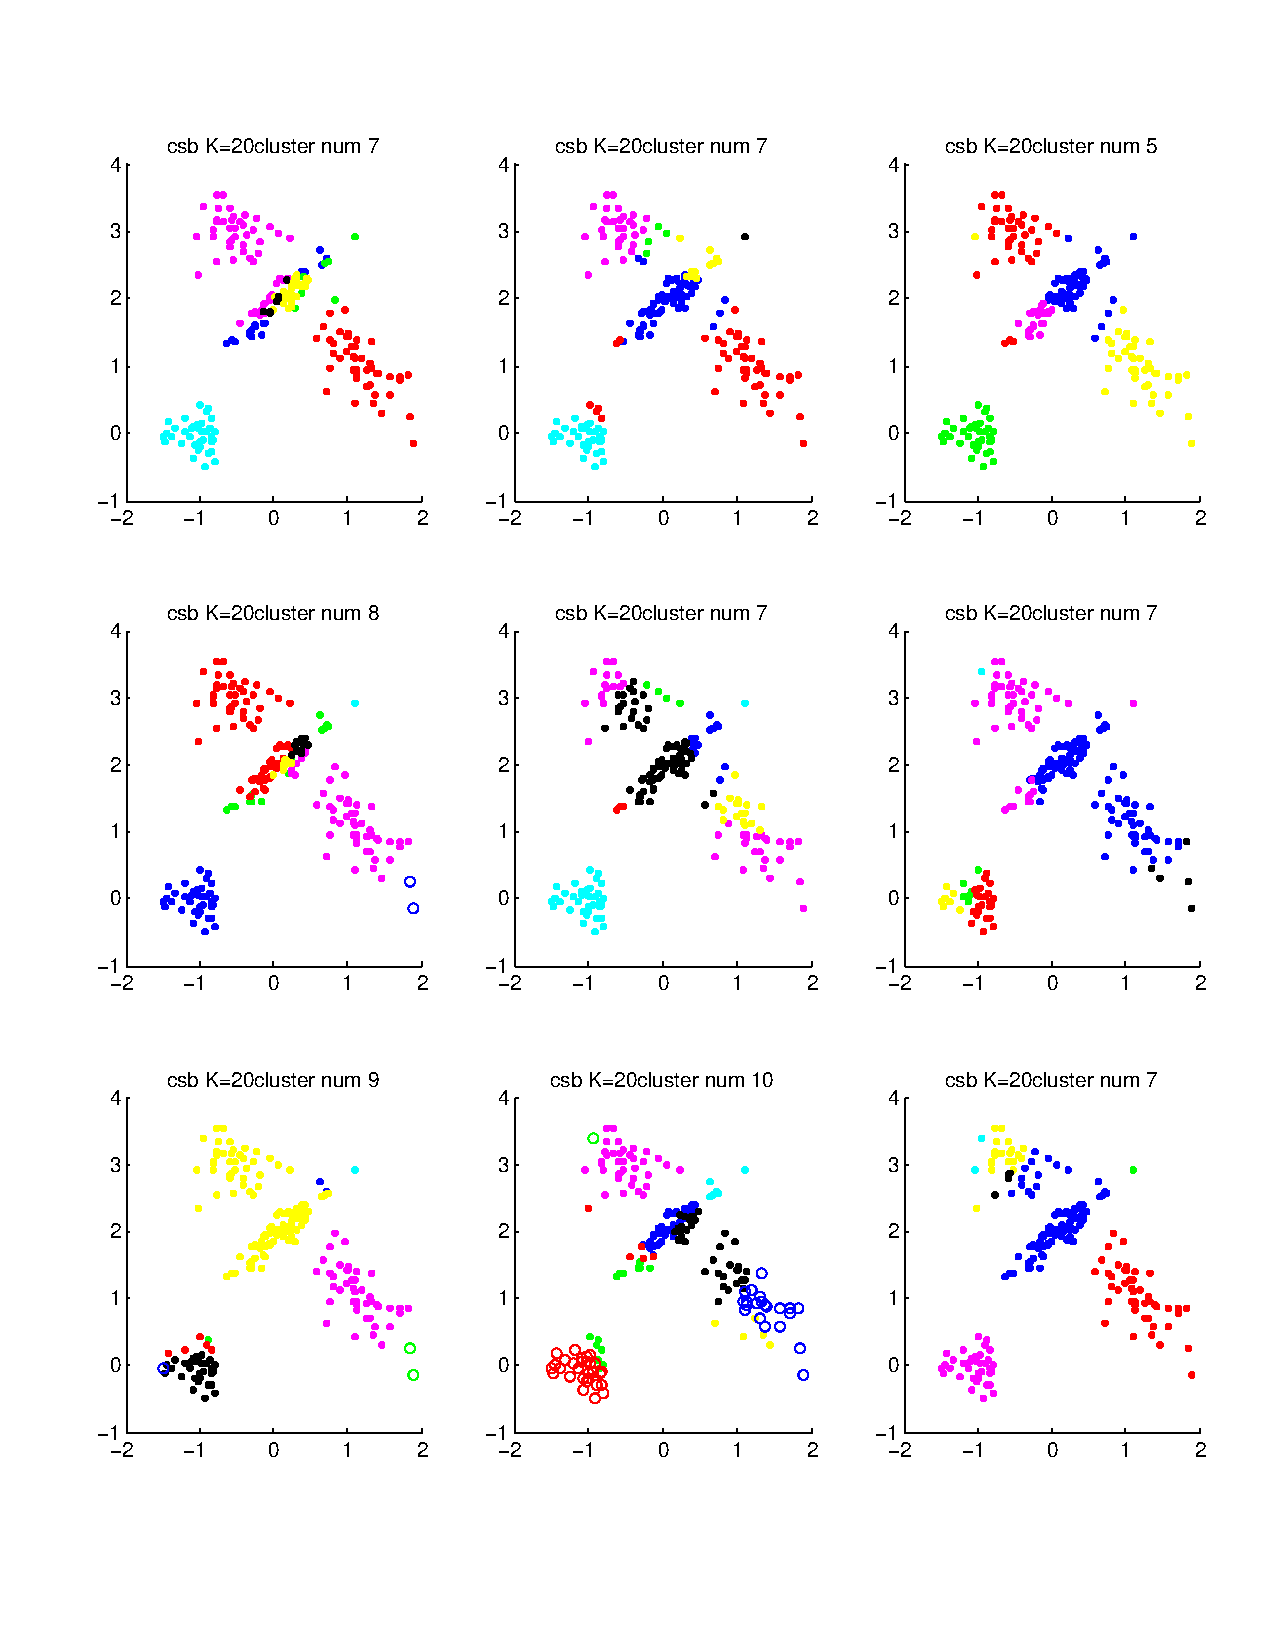
\includegraphics[width=5in,height=4.25in]{0_cee_20.pdf} \\
\end{center}


\subsection{1.3 Prior 2 (default EE)}
Differences:\\
$\phi_{0}$=1\\
$\eta_{0}$=3\\
\underline{$\xi_{0}$=0.01}\\
\underline{$B_{0}=\eta_{0}\xi_{0}$max(eig(S))*D*eye(D)=[0.033,0;0,0.033]} \\
\\The change of $B_{0},\xi_{0}$ that control the shape of the cluster matter significantly.

\begin{table}[t]
\caption{Prior 2 (with mean and std)}
\begin{center}
\begin{tabular}{|l|l|l|l|}

\hline
{\bf Learning Algorithm} &{\bf Initial Cluster Numbers} &{\bf Number of clusters}  &{\bf RandIndex} \\ 
\hline 
\multirow{2}{*}{EE(sampled initialization)} & 10 & 4.1(0.3) & 0.99(0.00) \\
					    & 20 & 4.1(0.3) & 0.99(0.00)\\
\hline
\multirow{2}{*}{EE(random initialization)}  & 10 & 6.9(1.2)&  0.97(0.01) \\
					    & 20 & 7.6(1.8)&  0.96(0.03) \\
\hline
\multirow{2}{*}{Collapsed EE}               & 10 & 5.6(1.6)&  0.90(0.22) \\
					    & 20 & 8.1(1.6)&  0.87(0.08) \\
\hline
\multirow{6}{*}{ME}                         & 1(Top-down) &    4  &  1 \\
					    & 200(Bottom-up) & 4  &  1 \\
					    & 200(Local search,1-200 update) & 29 &  0.77  \\
					    & 200(..+Merge) & 4   &  1 \\
					    & 200(Local search,random update) & 29.7(1.49)&  0.77(0.01) \\
					    & 200(..+Merge) & 4(0)&  1(0) \\
\hline
\end{tabular}
\end{center}
\end{table}

\begin{center}
Prior 2: ME,1-200 update, first 14 clusters \\
    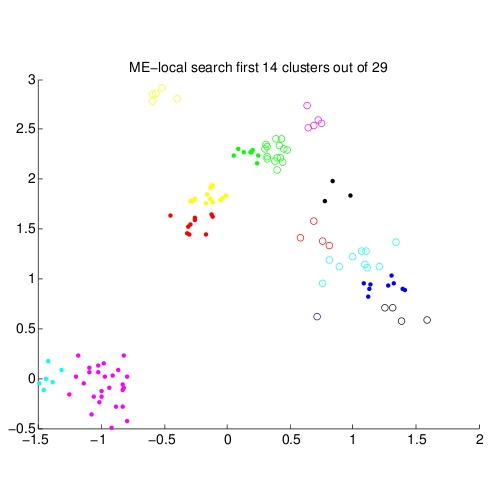
\includegraphics[width=4in,height=3.7in]{1_me_1.jpg} \\ 
Prior 2: ME,random update\\
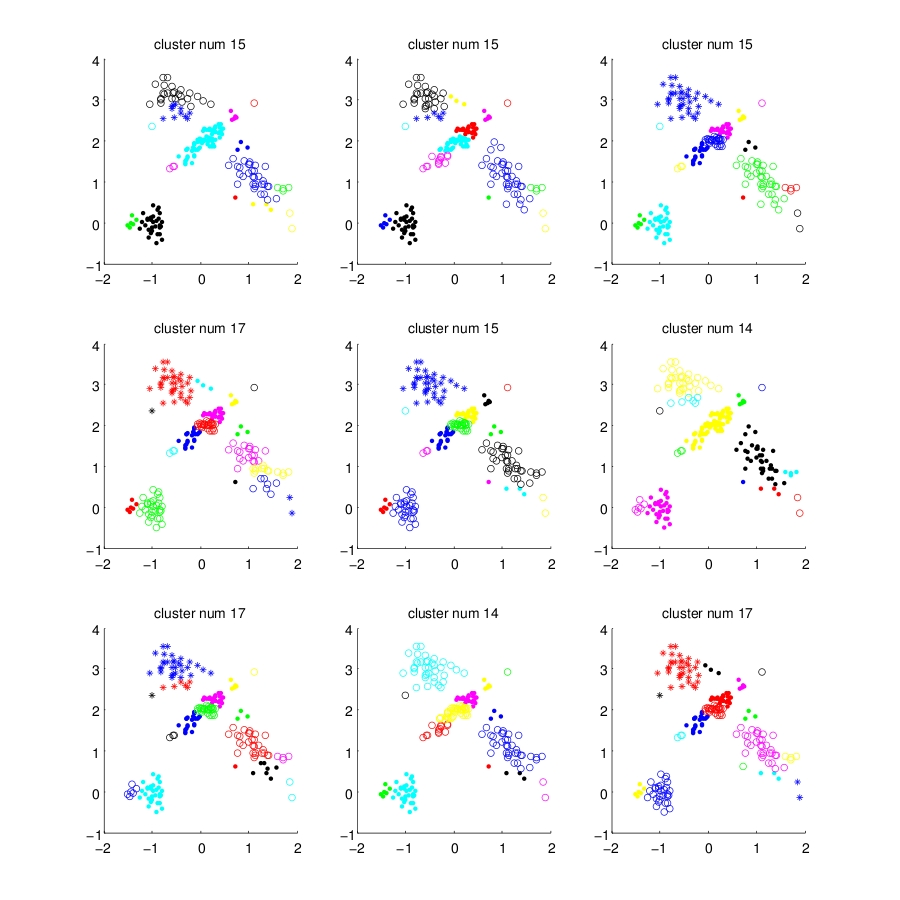
\includegraphics[width=6in,height=4.25in]{1_me_r.jpg} \\
Prior 2: EE,sis=0,K=20\\
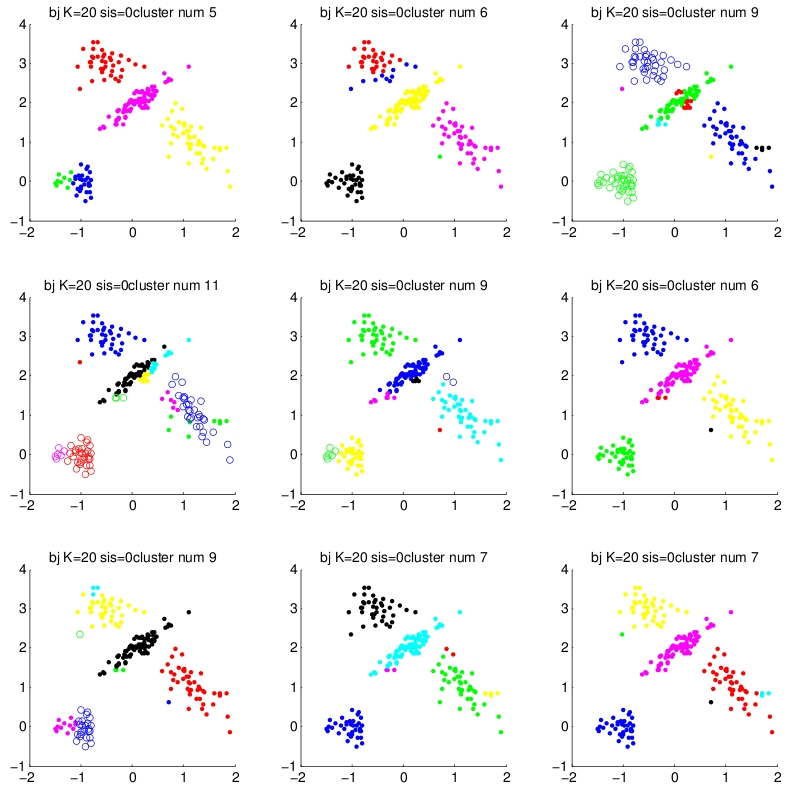
\includegraphics[width=5in,height=4.25in]{1_ee_20.jpg} \\
Prior 2: c-EE,K=20\\
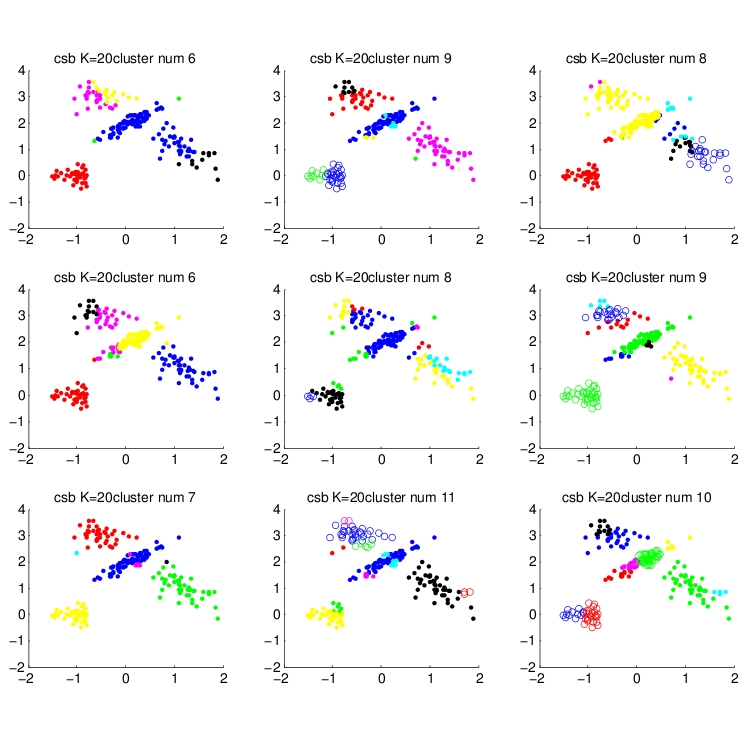
\includegraphics[width=5in,height=5in]{1_cee_20.jpg} \\

   \end{center}

\subsection{1.3 So, what's the matter}

\begin{center}
\begin{table}[t]
\begin{minipage}[b]{0.5\textwidth} 
\caption{Change from Prior 1 to 2}
\begin{tabular}{|l|l|l|}
\hline
{\bf parameter}  &{\bf $\sharp$ clusters}  &{\bf RandIndex} \\ 
\hline 
$\xi_{0}$  & 8 & 0.88 \\
\hline
$\eta_{0}$  & 10 & 0.87 \\
\hline
$\phi_{0}$  & 6 & 0.91 \\
\hline
$B_{0}$  & 17 & 0.81 \\

\hline
\end{tabular}
\end{minipage}
\begin{minipage}[b]{0.5\textwidth} 
\caption{Change from Prior 2 to 1}
\begin{tabular}{|l|l|l|}

\hline
{\bf parameter}  &{\bf $\sharp$ clusters}  &{\bf RandIndex} \\ 
\hline 
$\xi_{0}$  & 18 & 0.80 \\
\hline
$\eta_{0}$  & 25 & 0.79 \\
\hline
$\phi_{0}$  & 29 & 0.77 \\
\hline
$B_{0}$  & 10 & 0.87 \\
\hline
\end{tabular}
\end{minipage}

\end{table}
\end{center}
0) Empirical:(table 3 and 4)\\
i) Start from Prior 1, we change the parameter to Prior 2 one at a time:(update 1-200)\\ 
ii) Start from Prior 2, we change the different parameter back to Prior 1 one at a time:(update 1-200)\\ \\
1) Theoretical:\\
Different Prior $B_{0},\xi_{0}$ prefers different shape of the cluster.
Shown in the figure below, $B_{0}$ from Prior 1(right) is more sparse and elliptical than that from Prior 2(left)\\ 
Easily imagined,small $\xi_{0}$ will generate small clusters since $\mu_{c}$ is evaluated by $\mathcal{N}(\mu|m_{0},\xi_{0}\Omega)$\\
\begin{center}
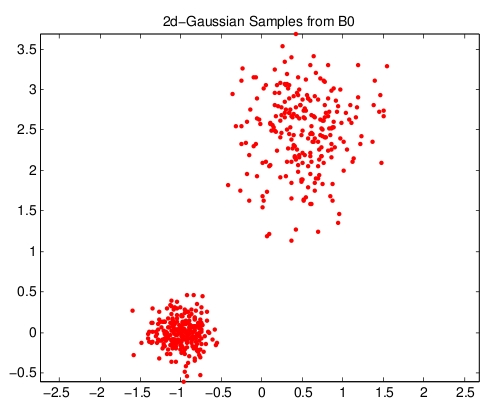
\includegraphics[width=3in,height=3in]{sample.jpg} \\
\end{center}

\section{2 CRF for HDP}
\subsection*{2.1 CRP for DPmixture}
One step back to derive the Allocation term $p(z_{1},...,z_{N}|\phi_{0})$ in the free energy with CRP.\\
Recall that \large {\bf  Free Energy:} \\
$\mathcal{F}([z],K_{+})=\sum_{c=1}^{K_{+}}[\frac{DN_{c}}{2}log\pi+\frac{D}{2}log\frac{\xi_{c}}{\xi_{0}}log det(B_{c})
-\frac{\eta_{0}}{2}log det(B_{0})-log \frac{\Gamma_{D}(\frac{\eta_{c}}{2})}{\Gamma_{D}(\frac{\eta_{0}}{2})}$\\
\ \  \underline{ $+\frac{1}{K_{+}}log \frac{\Gamma(N+\phi_{0})}{\Gamma(\phi_{0})} -log(\Gamma(N_{c}))-log \phi_{0}]$}\\
\\ \\ Known: N datas,K clusters, {$N_{i}$} datas in each cluster,$\phi_{0}$ for new cluster\\
 \\ Unknown: Cluster Assignment $z_{n}$\\
\\ \\ Allocation Term: \\
$p(z_{1},...,z_{N}|\phi_{0})=\Pi_{j=1}^{j=N}p(z_{j}|z_{1},...,z_{j-1},\phi_{0})$\\ \\
$p(z_{j}|z_{1},...,z_{j-1},\phi_{0})=\sum_{k=1}^{K(j)}\frac{m_{k(j)}}{j-1+\phi_{0}}\delta_{z_{j}=k}+\frac{\phi_{0}}{j-1+\phi_{0}}\delta_{z_{j}=K(j)+1}$\\ \\
1) Partition:$\Pi_{j=1}^{j=N}\frac{1}{\phi_{0}+j-1}=\frac{\Gamma(\phi_{0})}{\Gamma(N+\phi_{0})}$\\ \\
2) Forming new clusters:$\phi_{0}^{K}$\\ \\
3) Accumulating for all clusters:$\Pi_{j=1}^{j=N}(N_{j}-1)!=\Pi_{j=1}^{j=N}\Gamma(N_{j})$\\ \\
So,$-log(p(z_{1},...,z_{N}|\phi_{0}))=\sum_{c=1}^{K}\underline{ +\frac{1}{K}log \frac{\Gamma(N+\phi_{0})}{\Gamma(\phi_{0})} -log(\Gamma(N_{c}))-log \phi_{0}}\\$ \\
\subsection*{2.2 CRF for HDP}
Here, for the Gaussian case:\\
$\lambda=(m_{0},B_{0},\eta_{0},\xi_{0})$\\
$\theta_{k}=(\mu_{k},\Omega_{k})$\\ \\

Known: \\
1) Global: J Restaurants, K global dishes, T tables, N datas,\\
$t_{ji}:$ the table that customer i in Restaurant j sits;\\
$k_{jt}:$ the dish that table t in Restaurant j serves;\\
$\vec k:$ new dish different from what has been served;\\
$\vec t:$ the table different from what has been occupied;\\
2) Counting so far (during the process)\\
$m_{jk}:$ number of tables in Restaurant j serving dish k;\\
$m_{.k}:$ number of tables serving dish k;\\
$m_{j.}:$ number of tables in Restaurant j;\\
$m_{..}:$ number of tables;\\
$n_{jtk}:$ number of customers in Restaurant j at table t eating dish k;\\
$n_{jt.}:$ number of customers in Restaurant j at table t;\\
$n_{j..}:$ number of customers in Restaurant j;\\

Unknown: Table Assignment $t_{ji}$,Dish Assignment $k_{jt}$\\ 
Allocation Term: \\ \\
$p(k_{11},...,k_{JT_{J}}|\gamma)=\Pi_{j=1}^{J}(\Pi_{i=1}^{T_{j}}p(k_{ji}|\vec k_{1},...\vec k_{j-1},k_{j1},...,k_{j(i-1)},\gamma))$\\ \\
$p(t_{11},...,t_{JN_{J}}|\alpha)=\Pi_{j=1}^{J}(\Pi_{i=1}^{N_{j}}p(t_{ji}|t_{j1},...,t_{j(i-1)},\alpha))$\\ \\
$p(k_{jt}|\vec k_{1},...\vec k_{j-1},k_{j1},...,k_{j(t-1)},\gamma)=\sum_{k=1}^{K}\frac{m_{.k}}{m_{..}-1+\gamma}\delta_{k_{jt}=k}+\frac{\gamma}{m_{..}-1+\gamma}\delta_{k_{ji}=\vec k}$\\ \\
$p(t_{ji}|t_{j1},...,t_{j(i-1)},\alpha)=\sum_{t=1}^{m_{j.}}\frac{n_{jt.}}{i-1+\alpha}\delta_{t_{ji}=t}+\frac{\alpha}{i-1+\alpha}\delta_{t_{ji}=\vec t}$\\ \\

1) Partition:\\
k:\ $\Pi_{w=1}^{\sum_{j=1}^{J}m_{j.}}\frac{1}{\gamma+w-1}=\Pi_{w=1}^{m_{..}}\frac{1}{\gamma+w-1}=\frac{\Gamma(\gamma)}{\Gamma(T+\gamma)}$\\ \\
t:\ $\Pi_{j=1}^{J}\Pi_{i=1}^{i=n_{j..}}\frac{1}{\alpha+i-1}=\Pi_{j=1}^{j=J}\frac{\Gamma(\alpha)}{\Gamma(n_{j..}+\alpha)}$\\ \\

2) Forming new clusters (1st point in the cluster): \\
k: \ $\gamma^{K}$\\ \\
t: \ $\Pi_{j=1}^{J}\alpha^{m_{j.}}$\\ \\

3) Accumulating for each clusters (other points in the cluster): \\

k: \ $\Pi_{k=1}^{k=K}(m_{.k}-1)!=\Pi_{k=1}^{k=K}\Gamma(m_{.k})$\\ \\
t: \ $\Pi_{j=1}^{j=J}\Pi_{t=1}^{t=m_{j.}}(n_{jt.}-1)!=\Pi_{j=1}^{j=J}\Pi_{t=1}^{t=m_{j.}}\Gamma(n_{jt.})$\\ \\

So,
\large {\bf  Free Energy:} \\
$\mathcal{F}([z])$\\ =\\
(Likelihood)$ \sum_{k=1}^{K} [\frac{D n_{..k}}{2}log\pi+\frac{D}{2}log\frac{\xi_{k}}{\xi_{0}}+\frac{\eta_{k}}{2}log det(B_{k})-\frac{\eta_{0}}{2}log det(B_{0})
-log \frac{\Gamma_{D}(\frac{\eta_{k}}{2})}{\Gamma_{D}(\frac{\eta_{0}}{2})}]$
\\
+
\\
(Allocation:)$\underline{\sum_{j=1}^{J}\sum_{t=1}^{m_{j.}}[\frac{1}{m_{j.}}log \frac{\Gamma(n_{j..}+\alpha)}{\Gamma(\alpha)} -log(\Gamma(n_{jt.})-log \alpha]+
 \sum_{k=1}^{K} [\frac{1}{K}log \frac{\Gamma(T+\gamma)}{\Gamma(\gamma)} -log(\Gamma(n_{..k})-log \gamma]}$
\\ \\
=\\
(t-term)$ \sum_{j=1}^{J}\sum_{t=1}^{m_{j.}}[\underline{\frac{1}{m_{j.}}log \frac{\Gamma(n_{j..}+\alpha)}{\Gamma(\alpha)} -log(\Gamma(n_{jt.})-log \alpha
+\frac{1}{J m_{j.}}log \frac{\Gamma(T+\gamma)}{\Gamma(\gamma)}]}$\\ \\
+(k-term)$\sum_{k=1}^{K} [\frac{n_{..k}D}{2}log\pi+\frac{D}{2}log\frac{\xi_{k}}{\xi_{0}}+\frac{\eta_{k}}{2}log det(B_{k})-\frac{\eta_{0}}{2}log det(B_{0})
-log \frac{\Gamma_{D}(\frac{\eta_{k}}{2})}{\Gamma_{D}(\frac{\eta_{0}}{2})}
-\underline{log(\Gamma(n_{..k})-log \gamma]}$\\
where:\\
$\xi_{k}=\xi_{0}+n_{..k}$\\
$m_{k}=\frac{n_{..k} \vec x_{(k_{jt_{ji}}=k)}+\xi_{0}m_{0}}{\xi_{k}}$\\
$\eta_{k}=\eta_{0}=n_{..k}$\\
$B_{k}=B_{0}+n_{..k}S_{k}+\frac{n_{..k}\xi_{0}}{\xi_{k}}(\vec x_{(k_{jt_{ji}}=k)}-m_{0})(\vec x_{(k_{jt_{ji}}=k)}-m_{0})^{T}$\\
$S_{k}: sample covariance$\\


\begin{center}
Graphical Model for HDP\\
    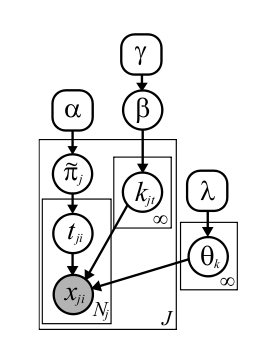
\includegraphics[width=4in,height=5in]{hdp.jpg} 
\end{center}



\section*{3. Search?}
The Key for ME algorithm is to search the optimanl assignment to minimize free energy.\\
\subsection*{3.1 Local Search}
It's kind of a black box since we put no prior on which datas could be in the same cluster. We just randomly throw one (or more) nodes into the black box 
and find the best assignment for it conditioning on others.
\subsection*{3.2 Search with Prior knowledge}
0) One step aside, considering the case of Linear Programming. Given a set of linear constraints of $x_{1},...x_{n}$, we want to find their
optimal "assignment" to maximize a linear object function. Without prior knowledge, the search is hopeless in $R^{n}$. But when we know that the constraints 
actually form a convex simplex with the optimal solution on some of the vertexes, the search becomes promising.\\
1) In our case, for mixture of Gaussian or image(later), there is the assumption of "Spatial Smoothness". \\
i) The Split and Merge technique implemented by Kurihara for ME DPmixture actually makes use of "Spatial Smoothness" from a top-down approach.
\\ Below is the matlab code for the heuristic split:\\

$\left[D,N\right] = size\left(data\right);\\
\left[ v,l \right] = eig\left( cov\left(data\right) \right);\\
\left[max\_val,max\_index\right] = max\left(diag\left(l\right)\right); \\
diff = v\left(:,max\_index\right)*sqrt\left(l\left(max\_index,max\_index\right)\right);\\
center = mean\left(data,2\right);\\
center1 = center + diff ;\\
center2 = center - diff ;\\
$
ii) From a bottom-up approach, we can make use K-nearest Neighbour or Density-based Clustering as an auxilary.
In each Group j, we can change datas that are "close" to each other as an $\alpha$ expansion.

\end{spacing}
\end{document}

%%%%%%%%%%%%%%%%%%%%%%%%%%%%%%%%%%%%%%%%%%%%%%%%%%%%%%%%%%%%%
